\documentclass[utf8x,hyperref={pdfpagelabels=false}]{beamer}

\usepackage[utf8x]{inputenc}
\usepackage[OT1]{fontenc}
\usepackage{amsmath,graphicx}
\usepackage{xcolor}
\usepackage{amsmath}
\usepackage{tikz}

\usetikzlibrary{arrows}
\usetikzlibrary{calc}

\usetheme{Malmoe}  % Now it's a beamer presentation with the lisa theme!        
\usecolortheme{beaver}
\setbeamertemplate{footline}[page number]
\setbeamertemplate{navigation symbols}{}
\mode<presentation>

\title{Recurrent Neural Networks in Theano}

\author{%
    \footnotesize
    \newline
    \newline
Phil\'{e}mon Brakel \newline
Institut des algorithmes d'apprentissage de Montréal \newline
Montreal Institute for Learning Algorithms \newline
Université de Montréal
}
\date{August 11th, Deep Learning Summer School 2015, Montréal}

\definecolor{termblue}{RGB}{51, 51, 179}
\newcommand{\term}[1]{\textcolor{termblue}{#1}}

\begin{document}

\begin{frame}[plain]
 \titlepage
 \vspace{-2em}
 \includegraphics[width=.8in]{mila.png}
 \hfill
 \includegraphics[width=.8in]{UdeM_logo}
\end{frame}

\setcounter{page}{1}

\section{Introduction}

\begin{frame}{Recurrent Neural Networks}
    Neural networks that can process sequences of inputs
    \begin{itemize}
        \item Used to process speech, language, music,\dots
        \item Recurrent Neural Networks are very powerful:
            \begin{itemize}
            \item Non-linear
            \item Distributed representations
            \item No Markov assumptions
            \end{itemize}
        \item However:
            \begin{itemize}
            \item Optimization can be challenging
            \item Learning \emph{long-term dependencies} is difficult
            \item Computations are not as easy to \emph{parallelize}
            \end{itemize}
    \end{itemize}
\end{frame}

\begin{frame}
    \frametitle{Standard Architecture}
    \begin{align*}
        h_t &= q(W_{xh}x_t + W_{hh}h_{t-1} + b_h)\\
        y_t &= r(W_{hy}h_{t} + b_y)
    \end{align*}
\begin{figure}[t]
\centering
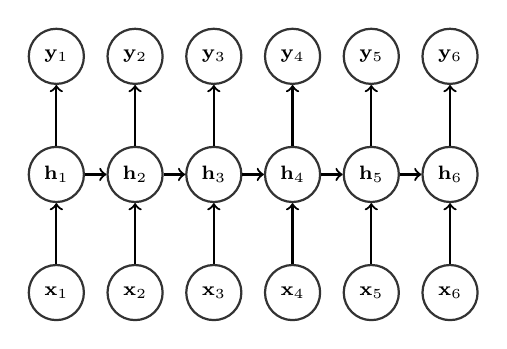
\begin{tikzpicture}[->,thick]
\scriptsize
\tikzstyle{main}=[circle, minimum size = 7mm, thick, draw =black!80, node distance = 12mm]
\foreach \name in {1,...,6}
    \node[main, fill = white!100] (y\name) at (\name,1.5) {$\mathbf{y}_\name$};
\foreach \name in {1,...,6}
    \node[main, fill = white!100] (h\name) at (\name,0) {$\mathbf{h}_\name$};
\foreach \name in {1,...,6}
    \node[main, fill = white!100] (x\name) at (\name,-1.5) {$\mathbf{x}_\name$};
\foreach \h in {1,...,6}
       {
        \path (x\h) edge (h\h);
        \path (h\h) edge (y\h);
       }
\foreach \current/\next in {1/2,2/3,3/4,4/5,5/6} 
       {
        \path (h\current) edge (h\next);
       }
    %\node[main] (G-\name) at (\x,0) {$\name$};
\end{tikzpicture}
\caption{A simple Recurrent Neural Network}
\end{figure}
\end{frame}


\begin{frame}
\frametitle{Long Short-Term Memory (LSTM)}
\begin{figure}[t]
\centering
\includegraphics[scale=.7]{lstmjozefowicz15}
\caption{LSTM: Learn long term dependencies by asserting control over what goes in and out of \emph{memory cells}.\footnotemark}
\end{figure}
\footnotetext{Figure Taken from Jozefowicz et al. (2015)}
\end{frame}

\begin{frame}
\frametitle{Long Short-Term Memory (LSTM)}
\begin{figure}[t]
\centering
\includegraphics[scale=1.0]{lstmgraves}
\caption{Another LSTM\footnote{Figure from Graves et al. (2013)}}
\end{figure}
\end{frame}

\begin{frame}
    \frametitle{Update Equations}
    \begin{align*}
        i_t &= \tanh(W_{xi}x_t + W_{hi}h_{t-1} + b_i)\\
        j_t &= \sigma(W_{xj}x_t + W_{hj}h_{t-1} + b_j)\\
        f_t &= \sigma(W_{xf}x_t + W_{hf}h_{t-1} + b_f)\\
        o_t &= \sigma(W_{xo}x_t + W_{ho}h_{t-1} + b_o)\\
        c_t &= f_t \otimes c_{t-1} + i_t \otimes j_t\\
        h_t &= \tanh(c_t) \otimes o_t
    \end{align*}
\end{frame}

\begin{frame}{RNNs can be Stacked}
\begin{figure}[t]
\centering
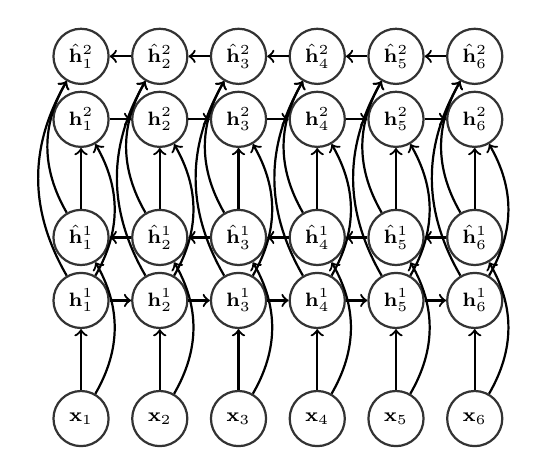
\begin{tikzpicture}[->,thick]
\scriptsize
\tikzstyle{main}=[circle, minimum size = 7mm, thick, draw =black!80, node distance = 12mm]
\foreach \name in {1,...,6}
    \node[main, fill = white!100] (l\name) at (\name,2.3) {$\mathbf{h}^2_\name$};
\foreach \name in {1,...,6}
    \node[main, fill = white!100] (k\name) at (\name,3.1) {$\hat{\mathbf{h}}^2_\name$};
\foreach \name in {1,...,6}
    \node[main, fill = white!100] (i\name) at (\name,.8) {$\hat{\mathbf{h}}^1_\name$};
\foreach \name in {1,...,6}
    \node[main, fill = white!100] (h\name) at (\name,0) {$\mathbf{h}^1_\name$};
\foreach \name in {1,...,6}
    \node[main, fill = white!100] (x\name) at (\name,-1.5) {$\mathbf{x}_\name$};
\foreach \h in {1,...,6}
       {
        \path (x\h) edge [bend right] (i\h);
        \path (x\h) edge (h\h);
        \path (i\h) edge [bend left] (k\h);
        \path (h\h) edge [bend right] (l\h);
        \path (h\h) edge [bend left] (k\h);
        \path (i\h) edge (l\h);
       }
\foreach \current/\next in {1/2,2/3,3/4,4/5,5/6} 
       {
        \path (i\next) edge (i\current);
        \path (h\current) edge (h\next);
        \path (k\next) edge (k\current);
        \path (l\current) edge (l\next);
       }
    %\node[main] (G-\name) at (\x,0) {$\name$};
\end{tikzpicture}
\caption{Two Bidirectional Recurrent Neural Networks stacked on top of each
other.}
\label{fig:birnn}
\end{figure}
\end{frame}

\section{RNNs In Practice}
\begin{frame}
    \frametitle{Parallelizing RNN computations}
    Apply RNNs to \emph{batches} of sequences\\
        Present the data as a 3D tensor of $(T \times B \times F)$.
        Each dynamic update will now be a matrix multiplication.
\begin{figure}
\centering
\resizebox{4cm}{2.5cm}{
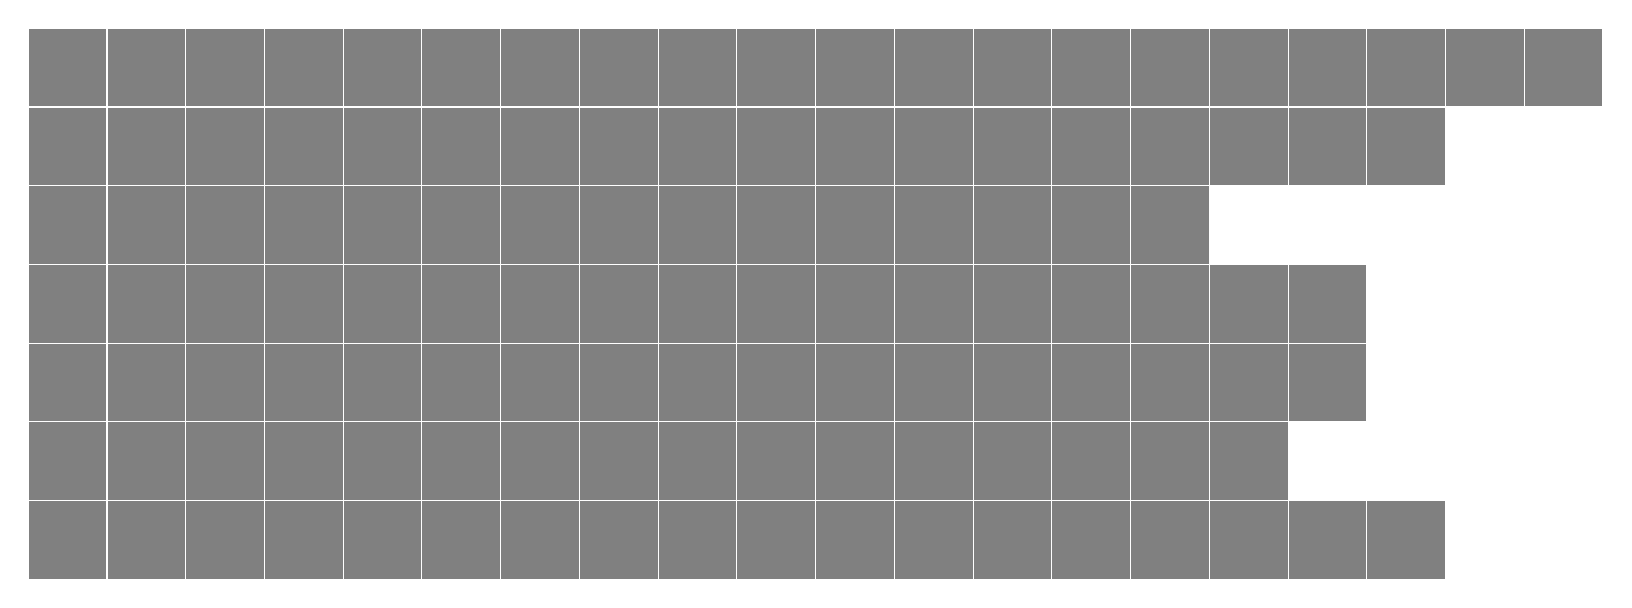
\begin{tikzpicture}
\tikzset{every cell/.style={draw=white}}
\tikzset{every cell 1/.style={fill=gray}}

   \foreach \row [count=\y] in {%
     {1,1,1,1,1,1,1,1,1,1,1,1,1,1,1,1,1,1,1,1},%
     {1,1,1,1,1,1,1,1,1,1,1,1,1,1,1,1,1,1,0,0},%
     {1,1,1,1,1,1,1,1,1,1,1,1,1,1,1,0,0,0,0,0},%
     {1,1,1,1,1,1,1,1,1,1,1,1,1,1,1,1,1,0,0,0},%
     {1,1,1,1,1,1,1,1,1,1,1,1,1,1,1,1,1,0,0,0},%
     {1,1,1,1,1,1,1,1,1,1,1,1,1,1,1,1,0,0,0,0},%
     {1,1,1,1,1,1,1,1,1,1,1,1,1,1,1,1,1,1,0,0}}
     \foreach \cell [count=\x] in \row  {
        \path [every cell/.try, every cell \cell/.try]
        (\x,-\y) rectangle ++(1,1);
       }
\end{tikzpicture}
}
\end{figure}
\end{frame}

\begin{frame}{Binary Masks}
    A \emph{mask} matrix may be used to aid with computations that ignore the padded zeros.
    In Theano this may be required to keep computations \emph{differentiable}.
\begin{figure}
\centering
\resizebox{8cm}{5cm}{
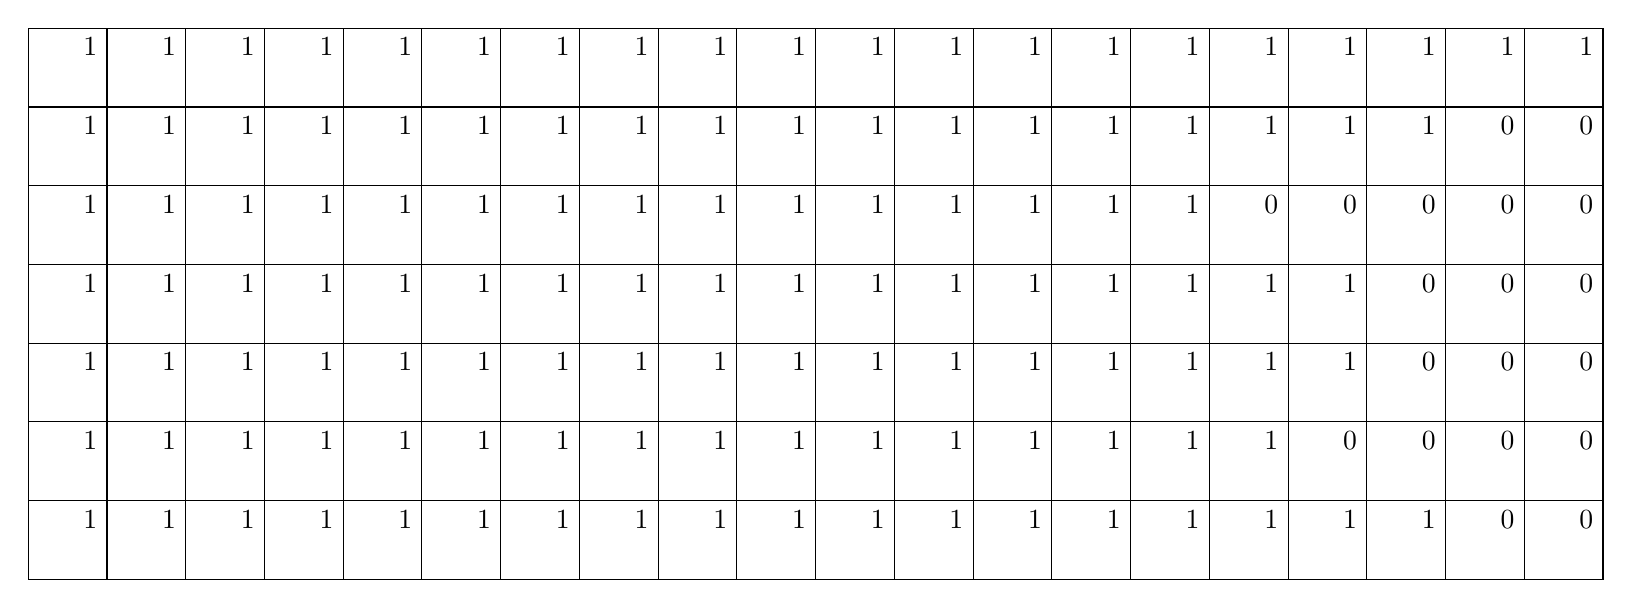
\begin{tikzpicture}
\tikzset{every cell/.style={draw=black}}
\tikzset{every cell 1/.style={draw=black}}

   \foreach \row [count=\y] in {%
     {1,1,1,1,1,1,1,1,1,1,1,1,1,1,1,1,1,1,1,1},%
     {1,1,1,1,1,1,1,1,1,1,1,1,1,1,1,1,1,1,0,0},%
     {1,1,1,1,1,1,1,1,1,1,1,1,1,1,1,0,0,0,0,0},%
     {1,1,1,1,1,1,1,1,1,1,1,1,1,1,1,1,1,0,0,0},%
     {1,1,1,1,1,1,1,1,1,1,1,1,1,1,1,1,1,0,0,0},%
     {1,1,1,1,1,1,1,1,1,1,1,1,1,1,1,1,0,0,0,0},%
     {1,1,1,1,1,1,1,1,1,1,1,1,1,1,1,1,1,1,0,0}}
     \foreach \cell [count=\x] in \row  {
        \path [every cell/.try, every cell \cell/.try]
        (\x,-\y) rectangle ++(1,1) node[below left] {$\cell$};
       }
\end{tikzpicture}
}
\end{figure}
\end{frame}

\begin{frame}{Binary Masks}
    It may be necessary to (partially) sort your data.
\begin{figure}
\centering
\resizebox{8cm}{5cm}{
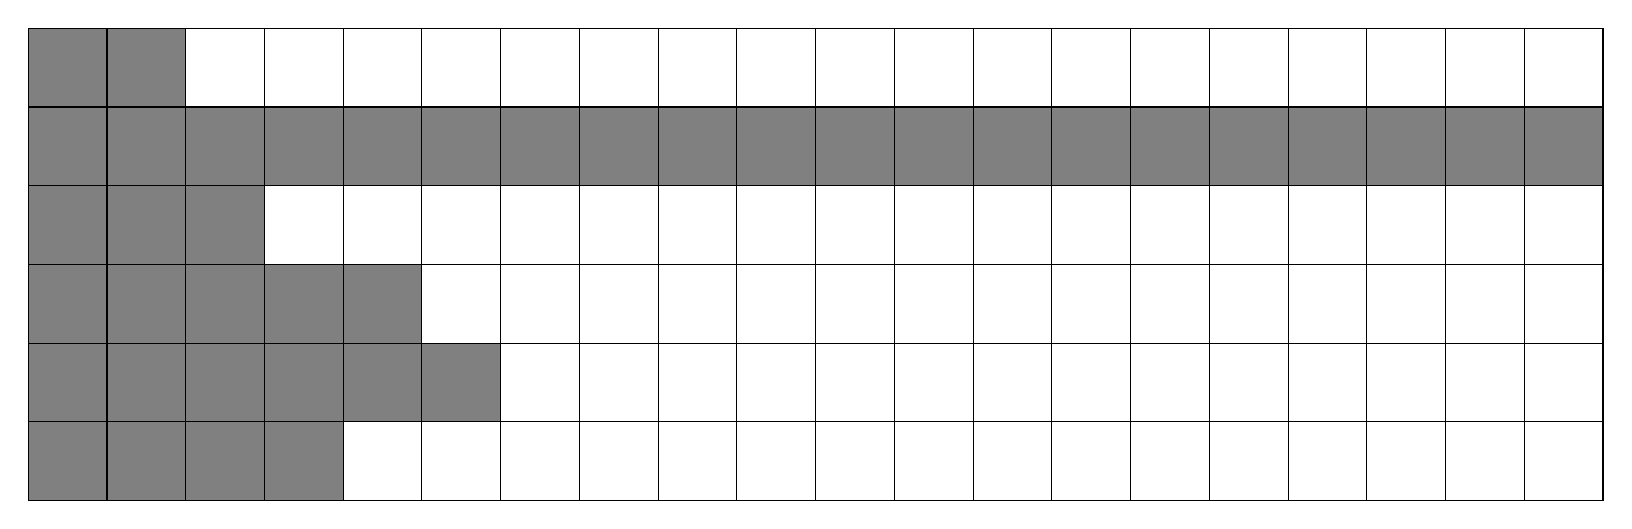
\begin{tikzpicture}
\tikzset{every cell/.style={draw=black}}
\tikzset{every cell 1/.style={fill=gray}}

   \foreach \row [count=\y] in {%
     {1,1,0,0,0,0,0,0,0,0,0,0,0,0,0,0,0,0,0,0},%
     {1,1,1,1,1,1,1,1,1,1,1,1,1,1,1,1,1,1,1,1},%
     {1,1,1,0,0,0,0,0,0,0,0,0,0,0,0,0,0,0,0,0},%
     {1,1,1,1,1,0,0,0,0,0,0,0,0,0,0,0,0,0,0,0},%
     {1,1,1,1,1,1,0,0,0,0,0,0,0,0,0,0,0,0,0,0},%
     {1,1,1,1,0,0,0,0,0,0,0,0,0,0,0,0,0,0,0,0}}
     \foreach \cell [count=\x] in \row  {
        \path [every cell/.try, every cell \cell/.try]
        (\x,-\y) rectangle ++(1,1);
       }
\end{tikzpicture}
}
\end{figure}
\end{frame}

\begin{frame}{Final Notes}
    \begin{itemize}
        \item<1-> Fuel has a transformer that automatically padds a batch of sequences and adds a mask
        \item<1-> Since masks are often used for multiplication, their type should often be floating point
        \item<1-> Be careful that your implementation doesn't nest \texttt{scan} nodes
        \item<2-> Have fun!
    \end{itemize}
\end{frame}


\end{document}
